\chapter{Die Turing-Welchman-Bombe}\label{ch:die-turing-bombe}

\section{Einführung}\label{sec:einfuerung_bombe}

Da frühe Verfahren zur Kryptoanalyse der Enigma-Maschine, wie zum Beispiel der \glqq Zyklometer\grqq{} oder die \glqq Bomba\grqq{}, durch die Einführung einer neuen Umkehrwalze (UKW-B), neuen Walzen und Änderung des Schlüsselverfahrens unbrauchbar gemacht wurden, musste ein neues Verfahren zur Kryptoanalyse der Enigma-Maschine von den Alliierten entwickelt werden. 
Der Durchbruch gelang, wie auch schon bei Marian Rejewski und seiner Bomba und Zyklometer, einem, beziehungsweise zwei Mathematikern.
Alan Turing und Gordon Welchman waren die Hauptverantwortlichen für die Entwicklung der \glqq Turing-Welchman-Bombe\grqq. 
Dieses Verfahren basiert ähnlich wie der Zyklometer auf \glqq Zyklen\grqq. 
Jedoch wurde hier nicht die Verdopplung des Spruchschlüssels im Spruchkopf ausgenutzt, sondern Zyklen zwischen einem an einer bestimmten Stelle im Geheimtext vermuteten Klartext (Crib) und dem Geheimtext bestimmt.
Die Turing-Welchman-Bombe testet immer eine Hypothese einer Steckerbrett-Verbindung und probierte mit drei von acht möglichen Walzen alle Walzenstellungen durch.
Auch wenn diese Hypothese sich als nicht korrekt erwies, findet die Turing-Welchman-Bombe bei korrekter Walzenlage durch Reductio ad absurdum trotzdem die gültigen Steckerbrett-Verbindungen.
Ziel war es die abgefangene Nachricht und ultimativ den Tagesschlüssel zu knacken.
Aufgrund der Einfachheit wird im Folgenden der Begriff \glqq Bombe\grqq{} anstelle von \glqq Turing-Welchman-Bombe\grqq{} verwendet.
\nopagebreak
\begin{figure}
	\centering
	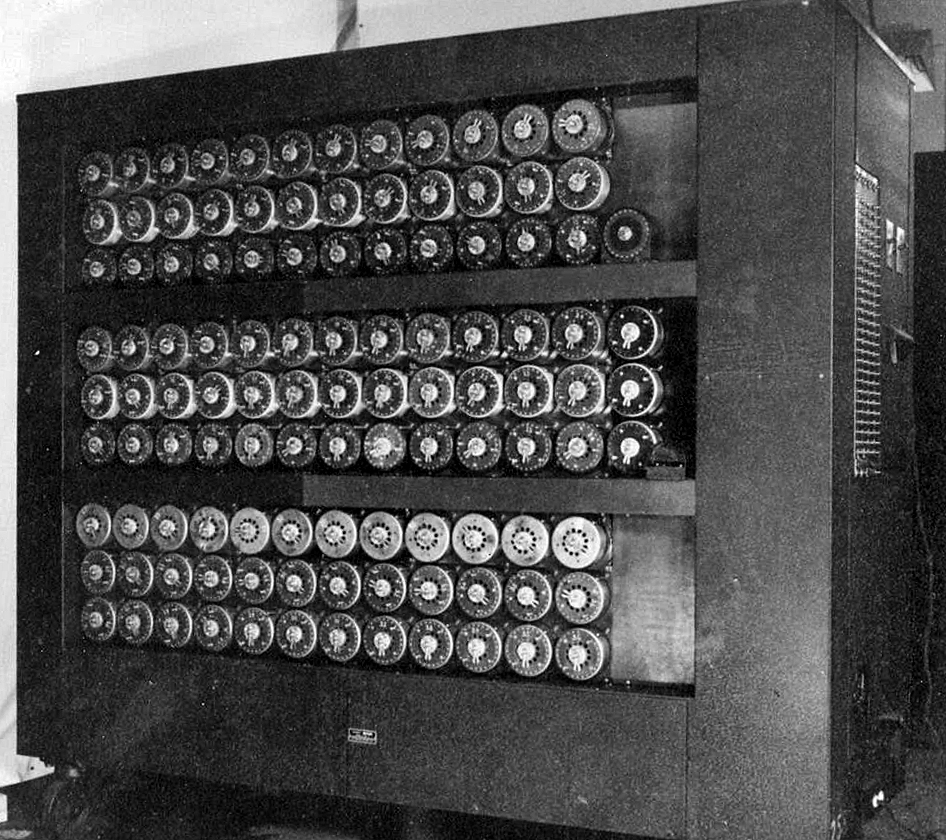
\includegraphics[width=0.4\linewidth]{Turing Bomb/BletchleyParkBombe}
	\caption{Eine Turing-Welchman-Bombe in Bletchley Park\autocite{wiki:bombe_picture}}
	\label{fig:bombe}
\end{figure}

\newpage

\section{Funktionsweise}\label{sec:funktionsweise_bombe}

\subsection{Vorbereitungen}\label{subsec:vorbereitungen}

\subsubsection{Crib}\label{subsubsec:crib}
Hier wird der Anglizismus \glqq Crib\grqq{} verwendet, da dieser Begriff keine richtige Deutsche Übersetzung hat.

Ein Crib ist ein Klartextfragment, welches an einer bestimmten Stelle im Geheimtext vermutet wird. 
Die deutsche Wehrmacht verwendete in den gesendeten Nachrichten häufig Floskeln. 
Ein Beispiel hierfür ist: \glqq Das Oberkommando der Wehrmacht gibt bekannt\grqq.
Nun musste das Crib positioniert werden.
Wie in~\cref{subsec:umkehrwalze} erklärt, ist es nicht möglich, dass ein Buchstabe auf sich selbst abgebildet wird.
Wurde eine mögliche Position gefunden, konnten die Mitarbeiter von Bletchley Park anfangen, das sogenannte Menü zu bauen.
Die~\cref{fig:positioning_crib} zeigt solch eine Positionierung.

\begin{figure}[htbp]
	\centering
	\caption{Positionierung des Cribs}
	\label{fig:positioning_crib}
	\resizebox{\linewidth}{!}{
		\ttfamily
		\begin{tabular}{|c|c|c|c|c|c|c|c|c|c|c|c|c|c|c|c|c|c|c|c|c|c|c|c|c|c|c|c|}
			\hline
			B & H & N & C & X & S & E & Q & K & O & B & I & I & O & D & W & F & B & T & Z & G & C & Y & E & H & Q & Q & J \\
			\hline
			O & B & E & R & K & O & M & M & A & N & D & O & D & E & R & \textcolor{red}{W} & E & H & R & M & A & \textcolor{red}{C} & H & T & & & &\\
			\hline
			\multicolumn{1}{|c|}{} & \textcolor{DarkGreen}{O} & \textcolor{DarkGreen}{B} & \textcolor{DarkGreen}{E} & \textcolor{DarkGreen}{R} & \textcolor{DarkGreen}{K} & \textcolor{DarkGreen}{O} & \textcolor{DarkGreen}{M} & \textcolor{DarkGreen}{M} & \textcolor{DarkGreen}{A} & \textcolor{DarkGreen}{N} & \textcolor{DarkGreen}{D} & \textcolor{DarkGreen}{O} & \textcolor{DarkGreen}{D} & \textcolor{DarkGreen}{E} & \textcolor{DarkGreen}{R} & \textcolor{DarkGreen}{W} & \textcolor{DarkGreen}{E} & \textcolor{DarkGreen}{H} & \textcolor{DarkGreen}{R} & \textcolor{DarkGreen}{M} & \textcolor{DarkGreen}{A} & \textcolor{DarkGreen}{C} & \textcolor{DarkGreen}{H} & \textcolor{DarkGreen}{T} & & & \\
			\hline
			\multicolumn{2}{|c|}{} & O & B & E & R & K & O & M & M & A & N & D & \textcolor{red}{O} & \textcolor{red}{D} & E & R & W & E & H & R & M & A & C & \textcolor{red}{H} & T & & \\
			\hline
			\multicolumn{3}{|c|}{} & \textcolor{DarkGreen}{O} & \textcolor{DarkGreen}{B} & \textcolor{DarkGreen}{E} & \textcolor{DarkGreen}{R} & \textcolor{DarkGreen}{K} & \textcolor{DarkGreen}{O} & \textcolor{DarkGreen}{M} & \textcolor{DarkGreen}{M} & \textcolor{DarkGreen}{A} & \textcolor{DarkGreen}{N} & \textcolor{DarkGreen}{D} & \textcolor{DarkGreen}{O} & \textcolor{DarkGreen}{D} & \textcolor{DarkGreen}{E} & \textcolor{DarkGreen}{R} & \textcolor{DarkGreen}{W} & \textcolor{DarkGreen}{E} & \textcolor{DarkGreen}{H} & \textcolor{DarkGreen}{R} & \textcolor{DarkGreen}{M} & \textcolor{DarkGreen}{A} & \textcolor{DarkGreen}{C} & \textcolor{DarkGreen}{H} & \textcolor{DarkGreen}{T} & \\
			\hline
			\multicolumn{4}{|c|}{} & O & B & \textcolor{red}{E} & R & \textcolor{red}{K} & \textcolor{red}{O} & M & M & A & N & \textcolor{red}{D} & O & D & E & R & W & E & H & R & M & A & C & H & T \\
			\hline
		\end{tabular}
	}
\end{figure}	

In Bletchley Park waren zudem viele Sprachexperten beschäftigt, die darauf spezialisiert waren, solche Cribs zu erstellen.
Dies erforderte sowohl sehr gute Kenntnisse über die Deutsche Sprache, als auch sehr gute Kenntnisse über die in~\cref{sec:uebertragung-der-nachrichten}
beschriebenen Regeln zu Funkspruch-Verschlüsselung.
Zudem mussten Eigenheiten und die \glqq Schreibfäule\grqq{} der Funker beachtet werden.
Ein Crib wurde unter der Vermutung benutzt, dass während der kompletten Eingabezeit des Abschnittes nur die rechte Walze (schnelle) Walze rotiert hat.
Aus diesem Grund darf ein Crib nicht länger als 25 Buchstaben sein, da sonst gewiss ein Übertrag auf die mittlere Enigma-Walze stattfand.
Die Bombe vernachlässigt also den Übertragzeitpunkt der Enigma-Walzen, wodurch die Ringstellung keine weitere Rolle spielt.
Um das Risiko zu minimieren, dass ein Übertrag stattgefunden hat, wurden meist Cribs mit einer Länge von ungefähr 13 Buchstaben verwendet.
In unserem Fall wäre also das Crib \glqq OBERKOMMANDODERWEHRMACHT\grqq{} zu lang.
Da das Crib jedoch keinen linguistischen Sinn ergeben muss, könnte man dies einfach zu \glqq OBERKOMMANDODER\grqq{} kürzen.

Eine Strategie der Alliierten für die Erzeugung von Cribs war zum Beispiel das sogenannte \glqq Gardening\grqq.
Damit ist das bewusste Provozieren von Funksprüchen, die einen bestimmten Klartext enthalten gemeint.
Eine Strategie war es, Seeminen in Flüsse, Häfen oder Seegebiete abzuwerfen.
Dafür musste ein Funker-Trupp in der Nähe des Ereignisses sein, welcher nicht verletzt werden durfte.
Ein mögliches Ziel war hier zum Beispiel ein Seegebiet in der Nähe eines U-Boots, da diese stets eine Enigma-Maschine an Bord hatten.
Nun beinhaltete der kurz darauf folgende Funkspruch mit einer hohen Sicherheit das Wort: \glqq Minen\grqq.

\newpage
\subsubsection{Menü}\label{subsubsec:menu}
Nun werden Buchstaben-Tupel zwischen Crib und Geheimtext gebildet.
An einem Beispiel von \glqq WETTERVORHERSAGE\grqq{} und \glqq SNMKGGSTZZUGARLV\grqq{} wären solche Tupel: \texttt{W:S}, \texttt{E:N} et cetera.
Nun werden die Tupel mit passenden Buchstaben aneinander gesetzt. 
In dem obigen Beispiel wären die Tupel unter anderem: $\texttt{W:S} - \texttt{S:V} - \texttt{V:E}$.
Der daraus resultierende Graph wird \glqq Menü\grqq{} genannt.
Er gibt die Einstellungen der Bombe vor.
\nopagebreak
\begin{figure}[htbp]
	\centering
	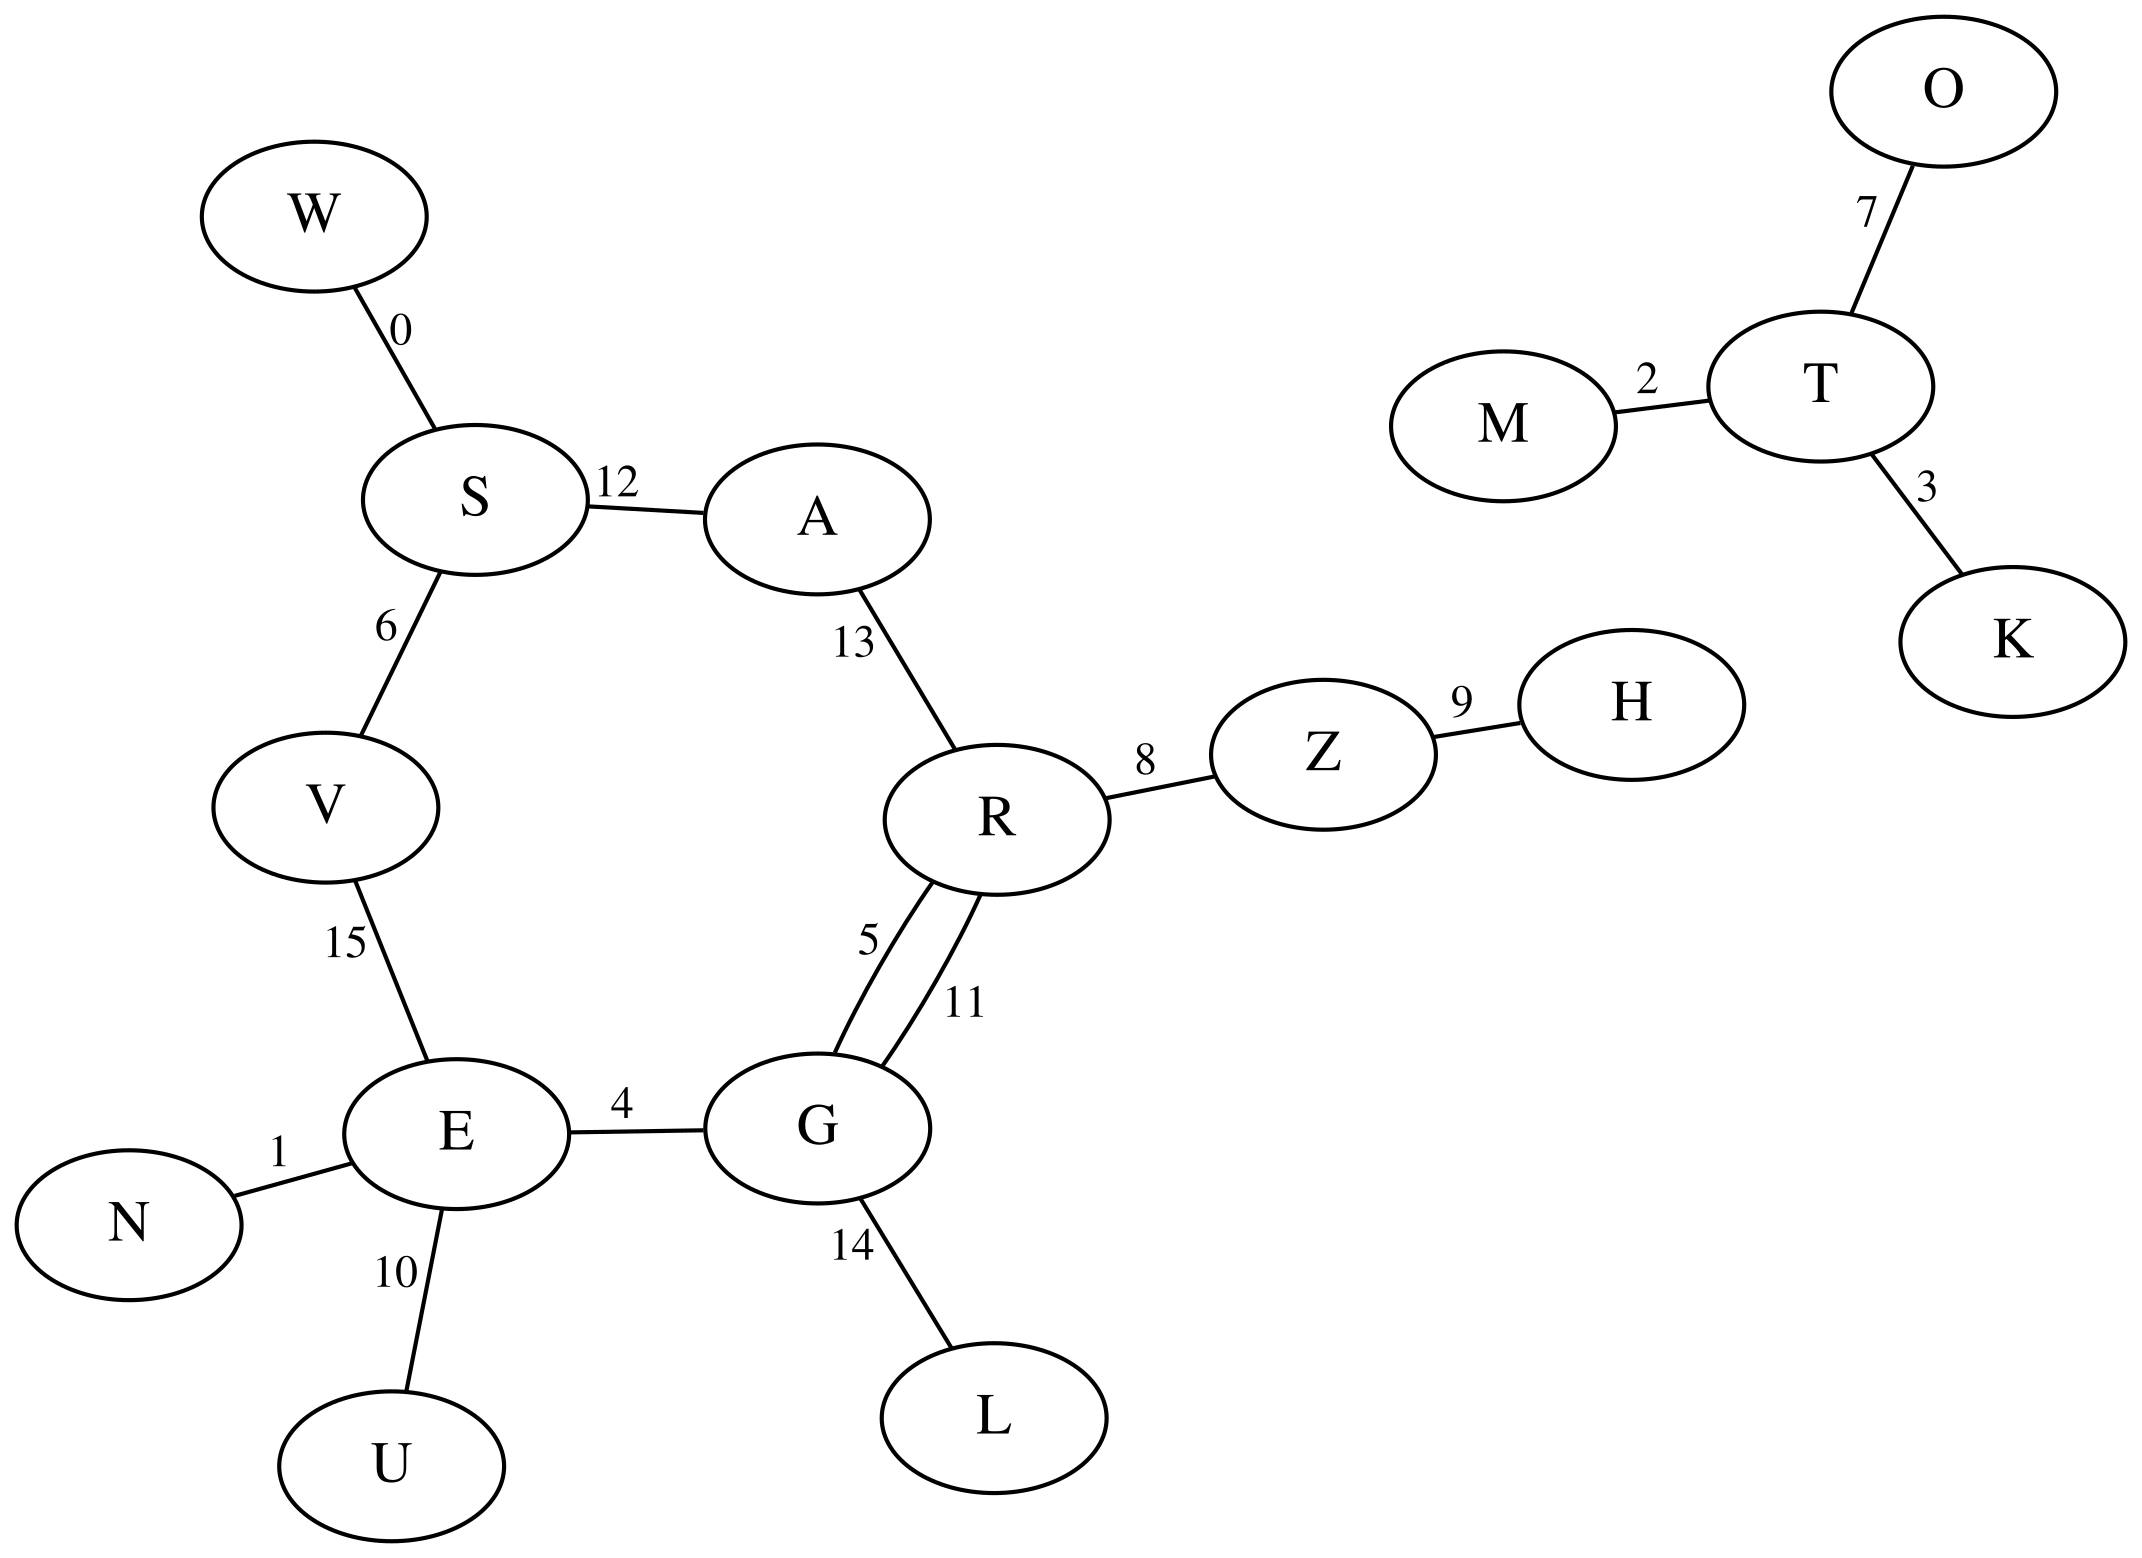
\includegraphics[width=.6\linewidth]{Turing Bomb/crib_cipher_cycle}
	\caption{Crib-Geheimtext Menü}
	\label{fig:crib_cipher_cycle}
\end{figure}

Wenn sich wie in~\cref{fig:crib_cipher_cycle} ein Zyklus bildet, ist dies eine brauchbare Crib-Geheimtext Kombination.
Alan Turing machte die Beobachtung, dass die Steckerbrett-Verbindungen der Enigma-Maschine keinen Einfluss auf den Verlauf des Menüs haben.
Dies ist durch die Eigenschaft des Steckerbrettes der Enigma-Maschine gegeben, welche eine monoalphabetische Substitution durchführt, die sich über den kompletten Chiffrierungs-Prozess nicht ändert.

Die Zahlen auf den Kanten geben hierbei die Position des Tupels innerhalb der gefundenen Crib-Geheimtext Kombination an.
Tupel wie 0, 1, 8, 9, 10 und 14 werden hier als \glqq Ausleger\grqq{} bezeichnet, da diese nicht aktiv zum Zyklus beitragen, aber trotzdem von Relevanz bei der Kryptoanalyse sind.
Aus Gründen, die später erläutert werden, sind Tupel-Kombinationen wie 5 und 11 äußerst effektiv für die Kryptoanalyse.
Tupel, die keinen Zyklus bilden, können ignoriert werden.
Somit sind die Tupel 2, 3 und 7 für den weiteren Verlauf der Kryptoanalyse irrelevant.


\newpage

\subsection{Scrambler}\label{subsec:scrambler}
Wie auch die Enigma-Maschine hat auch die Bombe \glqq Walzen\grqq.
Jedoch haben diese nicht 52, sondern 104 Kontakte, da es erforderlich war, diese miteinander zu verbinden.
Die Walzen der Bombe werden oft Scrambler genannt.

\begin{figure}[htbp]
	\centering
	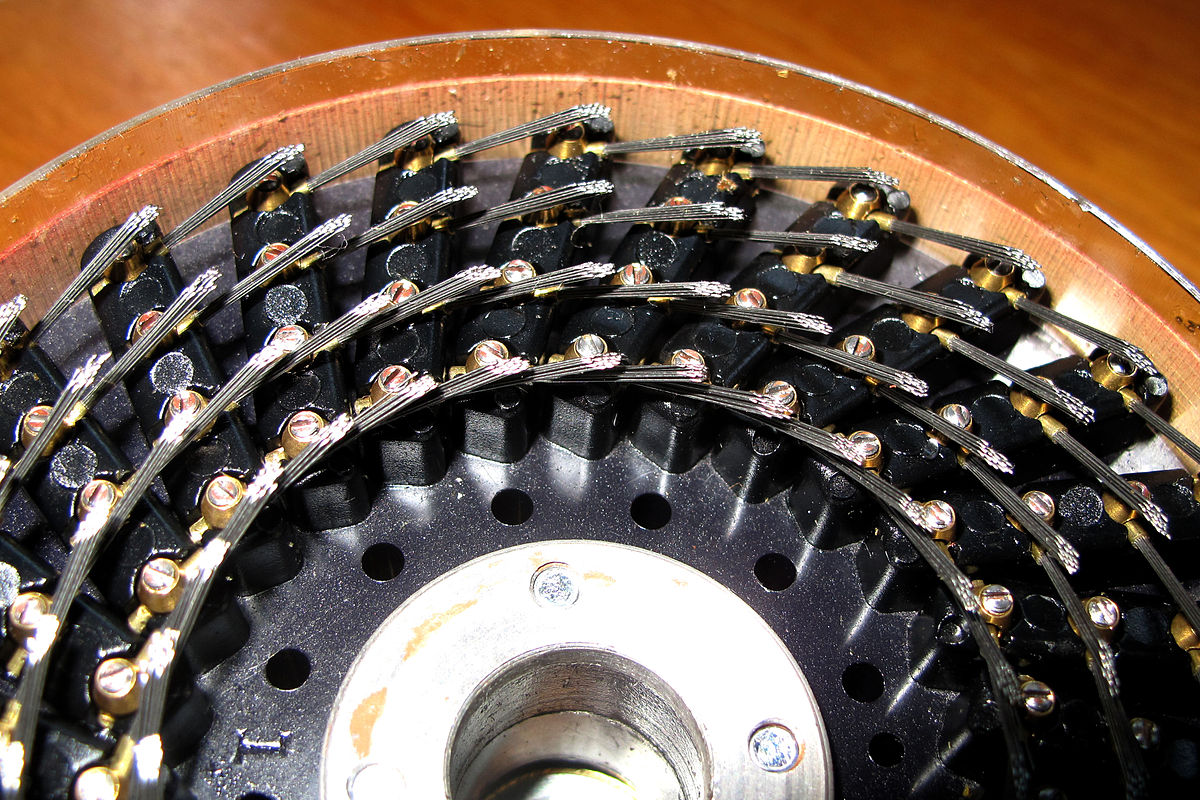
\includegraphics[width=0.4\linewidth]{Turing Bomb/WireBrushesOnBombeDrum}
	\caption{Die Kontakte der Scrambler\autocite{wiki:bombescrambler}}
	\label{fig:scrambler}
\end{figure} 


Die meisten Bomben bestanden aus dreimal zwölf Scramblersätzen.
Zwölf Scramblersätze ergeben eine \glqq Chain\grqq.
Ein Scramblersatz bestand aus drei Scrambler und simulierte eine Enigma-Maschine.
Der Grund, warum zwölf \glqq Enigmas\grqq{} parallel verwendet werden, ist, da somit eine komplette Ausgangsstellung der Walzen für das jeweilige Crib in einem Arbeitsgang überprüft werden kann.
Der unterste Scrambler eines Scramblersatzes repräsentiert die rechte, schnelle Walze einer Enigma-Maschine.
Der mittlere und oberste Scrambler ist repräsentativ für die mittlere und linke Walze der Enigma-Maschine.
Da die Scrambler keine Übertragskerbe besitzen, bewegt sich der nächste Scrambler immer nach einer vollen Rotation des aktuellen Scramblers, unabhängig von der Startposition.

Wurde nun durch die Mitarbeiter von Bletchley Park ein passendes Menü bestimmt, konnten die Scrambler in ihre Ausgangsstellung gebracht werden. 
Hierfür muss in dem Zyklus eine \glqq Route\grqq{} bestimmt werden.
Für den Zyklus in~\cref{fig:crib_cipher_cycle} könnte die Route lauten: \texttt{W $\to$ S $\to$ A $\to$ R $\to$ G $\to$ E $\to$ V $\to$ S}.

Die Zahlen auf den Kanten werden als \glqq Offsets\grqq{} für die untersten Walzen benutzt.
In unserem Beispiel sind also die Ausgangsstellungen der Scrambler also \texttt{AAA}, \texttt{AAL} und so weiter.
Sollen jetzt auch noch Ausleger, oder andere Tupel-Kombinationen wie 5 und 11 eingebunden werden, so können diese einfach an passender Stelle eingefügt werden: \texttt{AAD, AAE, AAK}.
Die Gesamtlänge der Elemente des Zyklus darf nicht zwölf überschreiten.

\subsection{Terminal}\label{subsec:terminal}
Auf der Rückseite der Bombe befinden sich dreimal 26 Terminal-Kontakte.
Ein 26er-Terminal-Satz ist jeweils einer Chain zugeordnet.
Jeder Kontakt in einem Terminal-Satz repräsentiert jeweils einen Buchstaben im Alphabet.
Jeder der 26 Kontakte hat 26 kleinere Kontakte, die wieder das Alphabet repräsentieren.
Wird nun im \emph{A}-Terminal an den \emph{e}-Kontakt Spannung angelegt, so wird die Hypothese getestet, dass der Geheimtext mit der Steckerbrett-Verbindung $A \Leftrightarrow E$ verschlüsselt wurde.

\subsection{In und Outs}\label{subsec:in_und_out}
Auf der Rückseite befinden sich Kontakte, die mit \glqq In\grqq{} und \glqq Out\grqq{} gekennzeichnet sind.
Wieder drei mal zwölf In- und Out-Paare, jeweils für die Scramblersätze.
Nun werden die Terminals mit den In und Outs verbunden.
Da der gewählte Routen-Startpunkt bei \glqq W\grqq{} liegt, wird der erste Scramblersatz auf das Offset \texttt{AAA} eingestellt.
Darauf wird das Terminal \emph{W} mit dem ersten In-Kontakt verbunden.
Der nächste Routen-Punkt \glqq S\grqq{} wird durch einen \glqq Brücken-Konnektor\grqq{} dem ersten Out mit dem zweiten In und dem Terminal \emph{S} verbunden.

\subsection{Diagonalbrett}\label{subsec:diagonalboard}
Gordon Welchman fiel auf, dass bei frühen Bomben nicht die Kommutativität des Steckerbretts beachtet wurde.
Ist $A$ mit $B$ gesteckert, so muss auch $B$ mit $A$ gesteckert sein.
Das Diagonalbrett stellte diese kommutativen Verbindungen her.
Für die Bombe heißt dies, dass wenn im \emph{A}-Terminal an den \emph{b}-Kontakt Spannung angelegt wird,
so auch der \emph{a}-Kontakt im \emph{B}-Terminal aktiv wird.
Dies trug maßgeblich zur Effizienz der Bombe bei.
Der Kontakt gleich dem Terminal-Buchstaben wird \glqq Self-Steckered\grqq{} genannt und stellt keine Steckerbrett-Verbindung dar.

\begin{figure}[htbp]
	\centering
	\caption{Diagonalbrett Verbindungen}
	\label{fig:diagonal_board_connections}
%	\begin{tikzpicture}[scale=0.7, every node/.style={scale=0.8}]
%		\foreach \i in {0,..., 4}{
%			\foreach \j in {0,..., 4}{
%				\fill (\i*1.5, \j*1.5) circle (2pt); 
%			}
%			\draw (\i*1.5, \i*1.5) circle (4pt);
%
%		}
%		
%		\foreach \i in {1,...,4}{
%			\foreach \j in {1,...,4}{
%				\node[below] at (\i*1.5, \j*1.5) {\char\numexpr97+\i};			
%			}
%		}
%		
%		\foreach \i in {1,..., 4}{
%			\node[left] at (0, \i*1.5) {\char\numexpr65+\i};
%			\node[below] at (\i*1.5, 0) {\char\numexpr65+\i};
%		}
%		
%		\node[below left] at (0,0) {A};
%		
%		
%	\end{tikzpicture}
	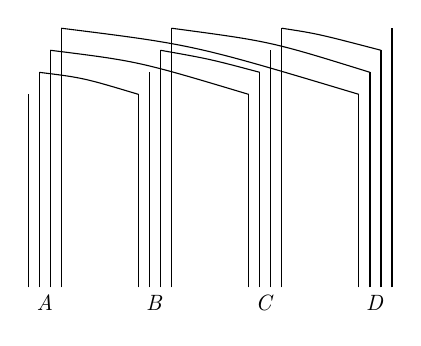
\begin{tikzpicture}[scale=0.7, every node/.style={scale=0.8}]
		
		%Säulen
		\foreach \i in {0,2,4,6} {
			\foreach \j in {0,0.2,0.4,0.6} {
				\draw[thin] (\i+\j,1.5) -- (\i+\j,5+\j*2);
			}
			\node[below] at (\i+0.3, 1.5) {\emph{\char\numexpr65+\i/2}};
		}
		
		
		%Querverbindungen
		\foreach \j in {0.2,0.4,0.6} {
			\draw[thin](\j,5+\j*2) .. controls (\j*5,5+\j*1.5) .. (\j*10,5);
		}	
		
		\foreach \j in {0.4, 0.6} {
			\draw[thin](\j+2,5+\j*2) .. controls ({(\j + 2 + \j*10 + 0.2)/2},5+\j*1.6) .. (\j*10+0.2,5.4);
		}
		
		\draw[thin](4.6,6.2) .. controls (5.25,6.1) .. (6.4,5.8);
		
		%TODO at A terminal
%		\draw[->] (-1,5.6) -- (0.2,5.4) node[left] at (-1,5.6) {\emph{b}-Kontakt im \emph{A}-Terminal};
	\end{tikzpicture}
\end{figure}



\subsection{Commons}\label{subsec:commons}
Sollen nun auch noch Ausleger oder andere Graphen-Konstrukte miteinbezogen werden, reicht ein In- und Out-Kontakt nicht aus.
Hierfür gibt es dreimal sechs Common-Kontaktblöcke à fünf Kontakte.
Commons-Kontakte sind blockweise mit CO1, CO2 et cetera gekennzeichnet.
Sechs Blöcke sind einer Chain zugeordnet.
Die Kontakte eines Blocks sind miteinander verbunden.
Somit ist es möglich, den Out-Kontakt des Scramblersatzes, der dem \glqq E\grqq{} in unserem Zyklus entspricht, mit Terminal \emph{V} und \emph{N} und den jeweiligen Ins der Scramblersätze zu verbinden. In~\cref{fig:bombe_rear} sind die Terminals, Commons und In und Outs mit den \glqq Brücken-Konnektoren\grqq{} zu sehen.
\nopagebreak
\begin{figure}[htbp]
	\centering
	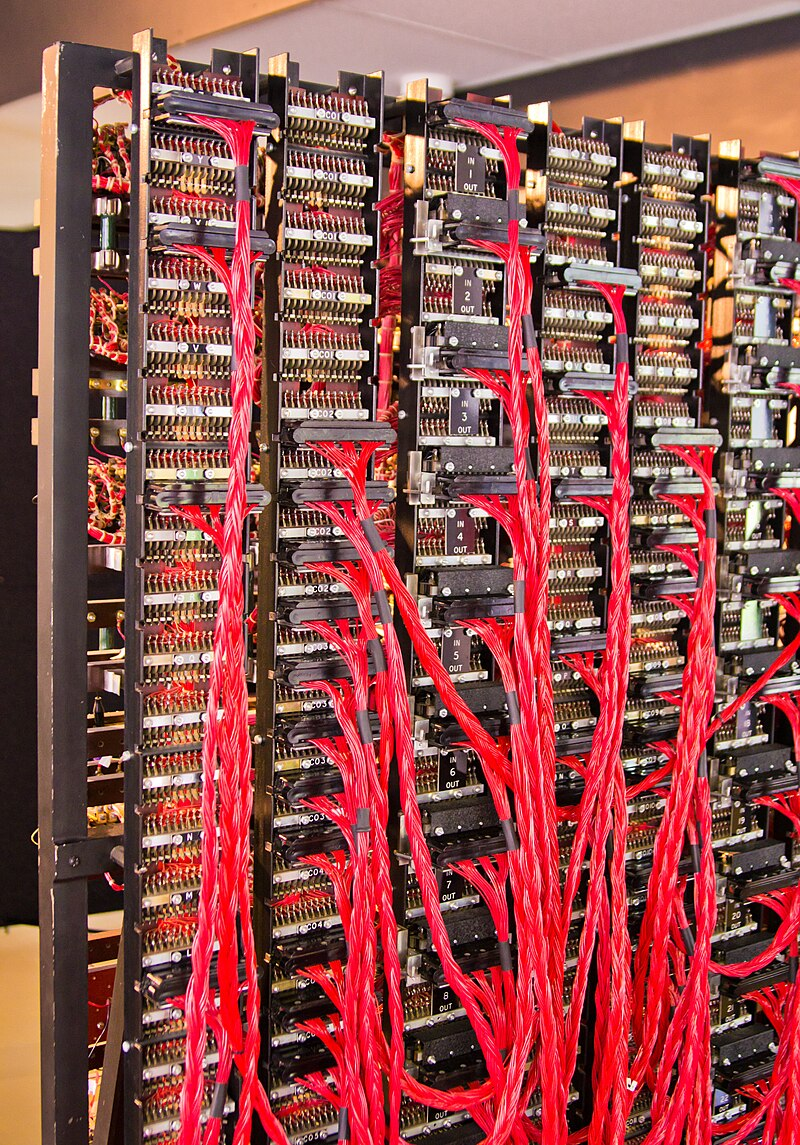
\includegraphics[width=0.5\linewidth, clip, trim=2cm 25cm 5cm 2cm]{Turing Bomb/Bletchley_Park_Bombe_Rear}
	\caption{Rückansicht der Bombe\autocite{wiki:bomberear}}
	\label{fig:bombe_rear}
\end{figure}
\newpage

\subsection{Test-Register}\label{subsec:test-register}
Um eine Steckerbrett-Verbindungs Hypothese zu testen, muss ein Test-Register bestimmt werden.
Dies sollte ein Buchstabe im Menü sein, der sehr viele Verbindungen hat.
In dem Fall von~\cref{fig:crib_cipher_cycle} wäre der Buchstabe \glqq G\grqq{} geeignet.
Nun muss ein Test-Buchstabe bestimmt werden.
Fällt die Wahl zum Beispiel auf \emph{A}, so wird die Hypothese der Steckerbrett-Verbindung $A \Leftrightarrow G$ getestet.
Es wird vermutet, dass während des Chiffrierungs-Prozesses die Steckerbrett-Verbindung $A \Leftrightarrow G$ benutzt wurde.

\begin{figure}[htbp]
	\centering
	\caption{Diagonalbrett Verbindungen mit Scrambler Verbindungen}
	\label{fig:diagonal_board_connections_w_scrambler}
	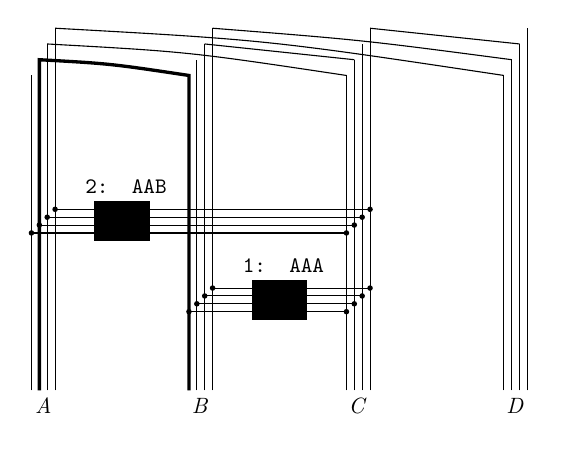
\begin{tikzpicture}[scale=1, every node/.style={scale=0.8}]
	
		
		%Säulen
		\foreach \i in {0,2,4,6} {
			\foreach \j in {0,0.1,0.2,0.3} {
				\draw[thin] (\i+\j,1) -- (\i+\j,5+\j*2);
			}
			\node[below] at (\i+0.15, 1) {\emph{\char\numexpr65+\i/2}};
		}
%		\draw[very thick] (2.2,1) -- (2.2,5.4);
		
		%		\draw[thin](0,9) .. controls (1,9.05) .. (2,9);
		
		%Querverbindungen
		\foreach \j in {0.1,0.2,0.3} {
			\draw[thin](\j,5+\j*2) .. controls (\j*10,5+\j*1.5) .. (\j*20,5);
		}	
		\draw[very thick] (0.1,1) -- (0.1,5.2) .. controls (1,5 + 0.1 * 1.5) .. (2,5) -- (2, 1);
		
		\foreach \j in {0.2, 0.3} {
			\draw[thin](\j+2,5+\j*2) .. controls ({(\j + 2 + \j*20 + 0.1)/2}, 5+\j*1.5) .. (\j*20 + 0.1, 5.2);
		}
		
		
		\draw[thin](4.3,5.6) .. controls (5.25,5.5) .. (6.2,5.4);
		
		\foreach \j in {0,0.1,0.2,0.3} {
			\draw[thin] (2+\j,2+\j) -- (4+\j,2+\j);
			\fill (2+\j,2+\j) circle (1pt);
			\fill (4+\j,2+\j) circle (1pt);
		}
		\fill (2.8, 1.9) rectangle (3.5, 2.4);
		\node[above] at (3.2, 2.4) {\texttt{1: AAA}};
		
		\foreach \j in {0,0.1,0.2,0.3}{
			\draw[thin] (\j, 3+\j) -- (4+\j, 3+\j);
			\fill (\j,3+\j) circle (1pt);
			\fill (4+\j,3+\j) circle (1pt);
		}
		
		\fill (0.8, 2.9) rectangle (1.5, 3.4);
		
		\node[above] at (1.2, 3.4) {\texttt{2: AAB}};
	\end{tikzpicture}
\end{figure}

In~\cref{fig:diagonal_board_connections_w_scrambler} wird die Hypothese der Steckerbrett-Verbindung $A \Leftrightarrow B$ getestet.
Unser Test-Register ist \emph{A}.
Es wurde ein Scramblersatz mit der Grundstellung \texttt{AAA} konfiguriert und Terminal \emph{B} mit dem ersten In und Terminal \emph{C} mit dem ersten Out verbunden.
Ein weiterer Scramblersatz wurde auf die Grundstellung \texttt{AAB} konfiguriert und dem zweiten In mit dem ersten Out, welcher durch den Brücken-Konnektor auch mit Terminal \emph{C} verbunden ist, verbunden.
Außerdem wurde das zweiten Out mit Terminal \emph{A} verbunden.
Die Tupel in~\cref{fig:diagonal_board_connections_w_scrambler} sind \texttt{B:C} an erster und \texttt{C:A} an zweiter Stelle. 
Da das Steckerbrett keinen Einfluss auf den Verlauf des Zyklus hat, spielt es keine Rolle, welche Hypothese getestet wird.
%Der Zyklus-Verlauf für~\cref{fig:diagonal_board_connections_w_scrambler} ist B $\rightarrow$ C $\rightarrow$ A\textellipsis.
Nun wird \emph{a} durch den Scramblersatz permutiert.
Ergibt sich durch die Permutation von \emph{a} ein anderer Buchstabe als \emph{c}, müsste die Steckerbrett-Verbindung signalisiert durch den aktiven Kontakt während der Chiffrierung benutzt worden sein.

Die Bombe hält in zwei Fällen:
\begin{enumerate}
	\item In dem Test-Register ist nach den Permutationen ein Kontakt aktiv – die Hypothese hat sich bewahrheitet.
	\item In dem Test-Register sind nach den Permutationen 25 Kontakte aktiv – die Hypothese ist falsch, aber die nicht aktiven Kontakte in den Terminals geben die \glqq richtige\grqq{} Steckerbrett-Verbindung an. (Reductio ad absurdum)
\end{enumerate}

Die anderen Fälle werden von der Bombe ignoriert.
Angenommen unser erster Scramblersatz permutiert das \emph{a} im \emph{B}-Terminal zu einem \emph{c} und unser zweiter Scramblersatz permutiert dieses \emph{c} zu einem \emph{d} im \emph{A}-Terminal, so erzeugt dies ein Widerspruch.
Es wurde die Hypothese der Steckerbrett-Verbindung $A \Leftrightarrow B$ aufgestellt, aber damit der dritte Buchstabe im Zyklus bei der aktuellen Walzenlage einem \emph{a} entsprechen kann, muss zusätzlich $A \Leftrightarrow D$ herrschen.
Dies ist eine widersprüchliche Aussage, da Buchstaben nur mit einem anderen verbunden sein können –- die Walzen rotieren.

Die Tupel-Kombinationen 5 und 11 in~\cref{fig:crib_cipher_cycle} sind besonders effektiv, da sich die Anzahl der aktiven Verbindungen rasch \glqq aufschaukelt\grqq.


